\chapter*{Introduction}

Les systèmes biologiques qui nous entourent présentent une incroyable diversité de structures leur permettant d'évoluer et de s'adapter à leur environnement par l'échange, le stockage et le traitement d'information.
Autrement formulé, ces systèmes biologiques présentent des capacités de calcul remarquables.
Ces mécanismes ont inspiré de nombreux algorithmes en informatique, imitant par exemple les colonies de fourmis, les essaims d'abeilles, les groupes de chats, les bancs de poissons ou encore les baleines, tous ces groupes d'animaux présentant des méthodes de communication décentralisées efficaces pour accomplir une tâche donnée~\parencite{Darwish2018BioinspiredCA}.
Un parangon de système biologique de calcul est sans conteste le cerveau, qui est capable d'exécuter des tâches de calcul et d'apprentissage incroyablement sophistiquées via une multitude de signaux électriques et chimiques circulant entre les neurones et dans les vaisseaux sanguins.
Cette inspiration biologique occupe une place de premier rang dans les débuts de la recherche en intelligence artificielle. Les premiers modèles d'apprentissage automatique ont été développés en s'appuyant sur des modélisations mathématiques de neurones biologique, afin de chercher à imiter les capacités d'évolution et d'adaptation à l'origine de l'apprentissage dans les réseaux de neurones biologiques.
Le perceptron s'appuyait par exemple sur un modèle simplifié de neurone biologique \parencite{McCulloch1990ALC}.
Les architectures de \emph{Deep Learning} qui en découlent se sont ensuite éloignées de la biologie pour s'extraire des contraintes physiques liées au neurone. Cette approche plus computationnelle a conduit à la création des architectures d'apprentissage performantes que nous connaissons aujourd'hui.
Néanmoins, la biologie, par sa diversité de comportements encore incompris, reste une source d'inspiration abondante pour apporter des paradigmes alternatifs ou complémentaires aux modèles d'apprentissage existants. Les possibilités d'inspiration biologique sont donc constamment en train d'évoluer.

De nombreuses modélisations générales du cortex cérébral, telles que~\cite{binzegger05, Meunier2009HierarchicalMI,sporns_structure_2013,betzel_multi-scale_2017} proposent que le cortex est une architecture composée de modules auto-organisés. Ces modules échangent des informations sensorielles collectées par l'organisme. Ces échanges sont réalisés de façon interne, liant des informations sensorielles et abstraites provenant de différentes parties du cortex et à différentes échelles spatiotemporelles. Enfin, bien qu'une hiérarchie de traitement de l'information apparaisse entre ces modules, certains traitant des entrées sensorielles et d'autres des entrées plus abstraites, de nombreux circuits de rétroactions entre les modules semblent présents à différents niveaux de l'architecture. 
Cette propriété de modularité est partagée par de nombreux systèmes biologiques et artificiels et présente des avantages en termes de réutilisation, de robustesse aux fautes, de redondance et de traitement local de l'information \parencite{clune_evolutionary_2013}.
Suivant ce constat, la recherche d'architectures cognitives s'inspirant de l'architecture du cortex cérébral est un enjeu de longue date dans la recherche en apprentissage automatique~\parencite{Kotseruba201840YO}. Il s'agit de développer des réseaux de neurones autonomes, capables de mémoire et de prise de décision de façon non supervisée, qui s'inspirent des architectures modulaires présentes dans le cerveau humain et qui cherchent à imiter certains comportements.
Le développement de la robotique et de l'apprentissage incarné appelle également à s'inspirer de telles architectures cognitives, qui sont directement liées à la perception sensorielle.
Un robot possède en effet de multiples capteurs, qui peuvent être défaillants, ou qui ne sont pas utilisés dans toutes les tâches que le robot doit effectuer. L'incorporation de mécanismes d'apprentissage au sein de tels agents doit prendre en compte l'aspect temporel et continu du flux de donnée entrant, ce qui appelle à la conception d'architecture d'apprentissage incluant des boucles sensorimotrices et capables de prise de décision autonomes.

Outre l'inspiration biologique liée à la structure corticale, la construction de systèmes d'apprentissage modulaires découle d'une motivation computationnelle.
Définissons plus précisément ce concept de modularité, qui peut prendre des significations très vastes, de l'informatique à la biologie. 
Dans une définition générale, un système modulaire est un système composé de sous-systèmes, les modules, qui peuvent être ajoutés ou supprimés sans impacter l'architecture des autres modules.
Cette vision générale de la modularité est l'approche classique privilégiée en sciences et ingénierie~: pour résoudre un problème, on le décompose en sous-problèmes, puis l'on développe des modules visant à résoudre chacun de ces sous-problèmes.
Nous nous plaçons dans une définition plus spécifique de cet aspect modulaire en s'intéressant uniquement à des architectures dont les modules communiquent entre eux de façon locale, sans être supervisés par un processus externe.
Cette vision de la modularité se rapproche plus de la vision biologique, dans laquelle aucun processus global ne vient a priori superviser l'organisation des systèmes. 


Nous pensons que cette approche modulaire est propice à faire émerger des nouveaux paradigmes d'apprentissage au sein d'architectures neuronales. 
Le comportement global du système résulte en effet de l'interaction entre les modules et non seulement de la somme des comportements des modules pris individuellement~: il s'agit de systèmes complexes. 
Des exemples de modèles artificiels ont exploré cette idée de modularité. Un exemple ancien en robotique autonome est l'architecture de \emph{sumsumption} de \cite{brooks_sumsumption_85}. Ces travaux construisent une architecture robotique composée de modules comportementaux simples, tels que \og marcher \fg{}, \og éviter un objet \fg{}, mais exploités en architecture par la présence de boucles de rétroaction. L'interaction de tous ces comportements de base permet au système de réagir de manière autonome à son environnement. 
Dans cet exemple, les modules ont une structure préétablie.
Nous centrons notre champ d'intérêt sur des architectures dont les modules sont a priori indifférenciés et interchangeables, et vont se spécialiser dans l'architecture au cours d'un l'apprentissage.
En résumé, nous entendons par architecture modulaire d'apprentissage une architecture composée d'une multiplicité de sous-systèmes indifférenciés, interchangeables et évoluant dans le temps.
Ils communiquent entre eux par une interface bien définie, et présentent des boucles de rétroaction, leur conférant un aspect dynamique. Cette interaction est traitée localement au sein des modules, sans supervision par un processus extérieur.

Nos travaux s'intéressent à un modèle d'apprentissage initialement inspiré de la biologie~: les cartes de Kohonen \parencite{Kohonen1982}.
Ces modèles sont caractérisés par leur capacité à représenter des données de façon ordonnée sur un espace de dimension plus faible (typiquement une ou deux dimensions).
L'algorithme d'apprentissage d'une carte auto-organisatrice suit un principe assez simple. Une carte est composée de vecteurs de l'espace d'entrée (prototypes) positionnés sur une grille de faible dimension.
Ils sont initialement distribués aléatoirement dans l'espace d'entrée. 
L'apprentissage est réalisé en présentant les entrées une à une à la carte, en trouvant leur \emph{Best Matching Unit} qui est le prototype le plus proche de l'entrée, puis en déplaçant ce prototype ainsi que ses voisins dans la grille vers l'entrée courante.
\`A l'issue de ce processus d'apprentissage, la grille munie des prototypes est dépliée sur l'espace d'entrée. N'importe quel vecteur de l'espace d'entrée peut être représenté par une position sur la grille.
Cette représentation spatiale fait des cartes de Kohonen un modèle simplifié de l'organisation spatiale observée dans les aires corticales.

La littérature autour des cartes de Kohonen est extrêmement fournie, en témoigne la bibliographie étendue réunissant 7717 travaux entre 1981 et 2005, réunie par \cite{Kaski1998BibliographyOS,oja_bibliography_2002,Honkela2009BIBLIOGRAPHYOS}.
Toutefois, elle s'est principalement attachée à l'augmentation des performances des cartes sur des applications d'apprentissage automatique et de fouille de données, comme de la compression d'image ou du clustering~\parencite{kohonen_essentials_2013}.
Nous pensons que leur inspiration biologique, leurs propriétés d'auto-organisation et de représentation en deux dimensions d'un espace complexe et la simplicité de leurs règles de mise à jour en font des candidates naturelles pour la création d'une architecture modulaire d'apprentissage.
D'une part, les cartes auto-organisatrices peuvent être vues comme un modèle très simplifié d'une aire corticale. Leur assemblage en architecture permettrait de pousser cette inspiration biologique au niveau de la structure corticale.
D'autre part, elles définissent une représentation en faible dimension de l'espace d'entrée, accessible par les positions dans la carte.
D'un point de vue computationnel, cette position se place comme une information peu coûteuse à échanger au sein d'une architecture.

L'idée d'architecture modulaire de cartes semble donc découler naturellement de la nature même de l'algorithme, et est d'ailleurs formulée par Kohonen dès 1995~:
\begin{quote}
\og Un objectif à long terme de l'auto-organisation est de créer des systèmes autonomes dont les éléments se contrôlent mutuellement et apprennent les uns des autres. De tels éléments de contrôle peuvent être implémentés par des SOMs spécifiques~; le problème principal est alors l'interface, en particulier la mise à l'échelle automatique des signaux d'interconnexion entre les modules et la collecte de signaux pertinents comme interface entre les modules. Nous laisserons cette idée aux recherches futures. \fg{}
(Traduit de \cite{Kohonen1995SelfOrganizingM})
\end{quote}

Depuis, bien que des travaux aient proposé des architectures de carte auto-organisatrices, peu ont effectivement exploré l'aspect spatialement ordonné et la simplicité des règles mise à jour des poids d'une carte pour les assembler en architectures modulaires comportant des rétroactions~: des architectures non-hiérarchiques.

Au vu des propriétés des cartes de Kohonen et de la littérature, nous proposons dans cette thèse de construire une architecture modulaire non-hiérarchique de cartes.
Notre démarche est constructive~: nous définissons un modèle de carte pouvant être utilisé en tant que module, puis nous cherchons expérimentalement à comprendre les comportements qui émergent de l'association des modules.
L'architecture que nous proposons va dans l'idée d'implémenter des mécanismes généraux liés à la cognition tels que l'apprentissage non-supervisé, autonome, le traitement de données temporelles, l'apprentissage sur le long terme et la fusion de données multimodales, s'inspirant du traitement multisensoriel du cerveau humain.
Cette problématique étant extrêmement vaste, nous avons choisi dans cette thèse de nous concentrer sur la tâche particulière d'apprentissage associatif de données multimodales. 
Il s'agit pour l'architecture d'apprendre des relations existant entre des entrées provenant de différents espaces, en plaçant cet apprentissage de relations à un niveau interne à l'architecture et non en concaténant les entrées avant de les présenter à l'architecture. Le but est d'apprendre à la fois une représentation des modalités et de leurs relations, tout en gardant une sémantique sur chaque modalité.

\begin{center}
  $\ast$
\end{center}

En résumé, cette thèse vise à répondre à deux problématiques principales entremêlées~: (i)~développer un modèle d'architecture non-hiérarchique de cartes auto-organisatrices exploitant l'aspect topographiquement ordonné de ce modèle d'apprentissage, et (ii)~élaborer une méthodologie expérimentale et des outils permettant de mettre en évidence et évaluer l'apprentissage associatif qui émerge d'une telle architecture.

\begin{center}
  $\ast$
\end{center}

Le manuscrit est organisé de la façon suivante.
Le chapitre~\ref{chap:architectures} présente un état de l'art des architectures de cartes auto-organisatrices existant dans la littérature. Ces modèles d'architectures sont issus de plusieurs domaines, de l'apprentissage automatique aux neurosciences computationnelles.
Le chapitre propose une revue des modèles principaux en s'attachant à unifier les notations et leurs désignations afin d'identifier les points communs et différences principales de conception de ces modèles.
Cet état de l'art nous permettra de situer le modèle que nous proposons au regard de la littérature existante.

Nous détaillerons au chapitre~\ref{chap:modele} le modèle d'architecture non-hiérarchique de cartes auto-organisatrices que nous développons et étudions dans cette thèse, que nous avons appelé CxSOM, pour \emph{Consensus-driven Multi-SOM}. Il s'inscrit dans la continuité de modèles développés dans notre équipe de recherche.
Nous définissons un modèle de carte qui peut être assemblé à volonté, de façon modulaire, en architecture non-hiérarchique. Ce modèle utilise la position du Best Matching Unit d'une carte comme seule interface entre les modules, rendant les activités des cartes interdépendantes. Pour gérer les rétroactions, l'apprentissage s'appuie sur une recherche de consensus entre les cartes pour la recherche d'un BMU.
Le chapitre~\ref{chap:relaxation} est une analyse plus approfondie de la recherche de consensus entre les cartes afin de valider ce mécanisme en tant qu'algorithme de choix de BMU pour l'apprentissage.

Si notre approche a pour but général de concevoir une architecture comportant de nombreux modules ainsi que des connexions temporelles, nous avons concentré cette thèse sur l'analyse expérimentale des comportements d'apprentissage associatif dans des architectures de deux et trois cartes.
Le pari de la construction d'une architecture modulaire est de faire émerger des nouveaux comportements, des nouveaux mécanismes de calcul~; aussi faut-il pouvoir les mettre en évidence. Nos travaux se sont vite confrontés à une difficulté de visualisation d'une telle architecture de cartes. Cette thèse met l'accent sur une méthodologie d'analyse expérimentale de cette architecture modulaire, ce qui nous permettra d'en tirer des comportements élémentaires qui serviront à poser les bases de la construction d'architectures plus complexes.
Nous introduisons au chapitre \ref{chap:repr} cette méthode expérimentale et un cadre de représentation des entrées, et proposons une définition de ce que signifie qu'une architecture de cartes encode les entrées et leurs relations.
Nous présentons ensuite au chapitre \ref{chap:analyse} les comportements élémentaires d'apprentissage associatif observés sur des architectures de deux et trois cartes en une dimension, à partir des représentations que nous avons proposées. Nous présenterons en particulier un comportement de prédiction d'entrée, rendu possible par les rétroactions et la dynamique de recherche du BMU présentes dans notre modèle.
Nous explorons au chapitre~\ref{chap:indicateur} des indicateurs numériques d'évaluation de l'apprentissage associatif par l'architecture de cartes, dans le but d'étendre l'analyse du modèle à des architectures plus grandes, qui seraient difficilement représentables graphiquement.
Le chapitre \ref{chap:analyse2D} étend enfin les mécanismes d'apprentissage que nous avons identifiés à des architectures de cartes en deux dimensions, se plaçant comme une étude préliminaire pour saisir la scalabilité du modèle.
Nous conclurons sur les perspectives de développement du modèle CxSOM que mettent en évidence nos travaux.

    \begin{figure*}[b]
        \vspace{1cm}
        \centering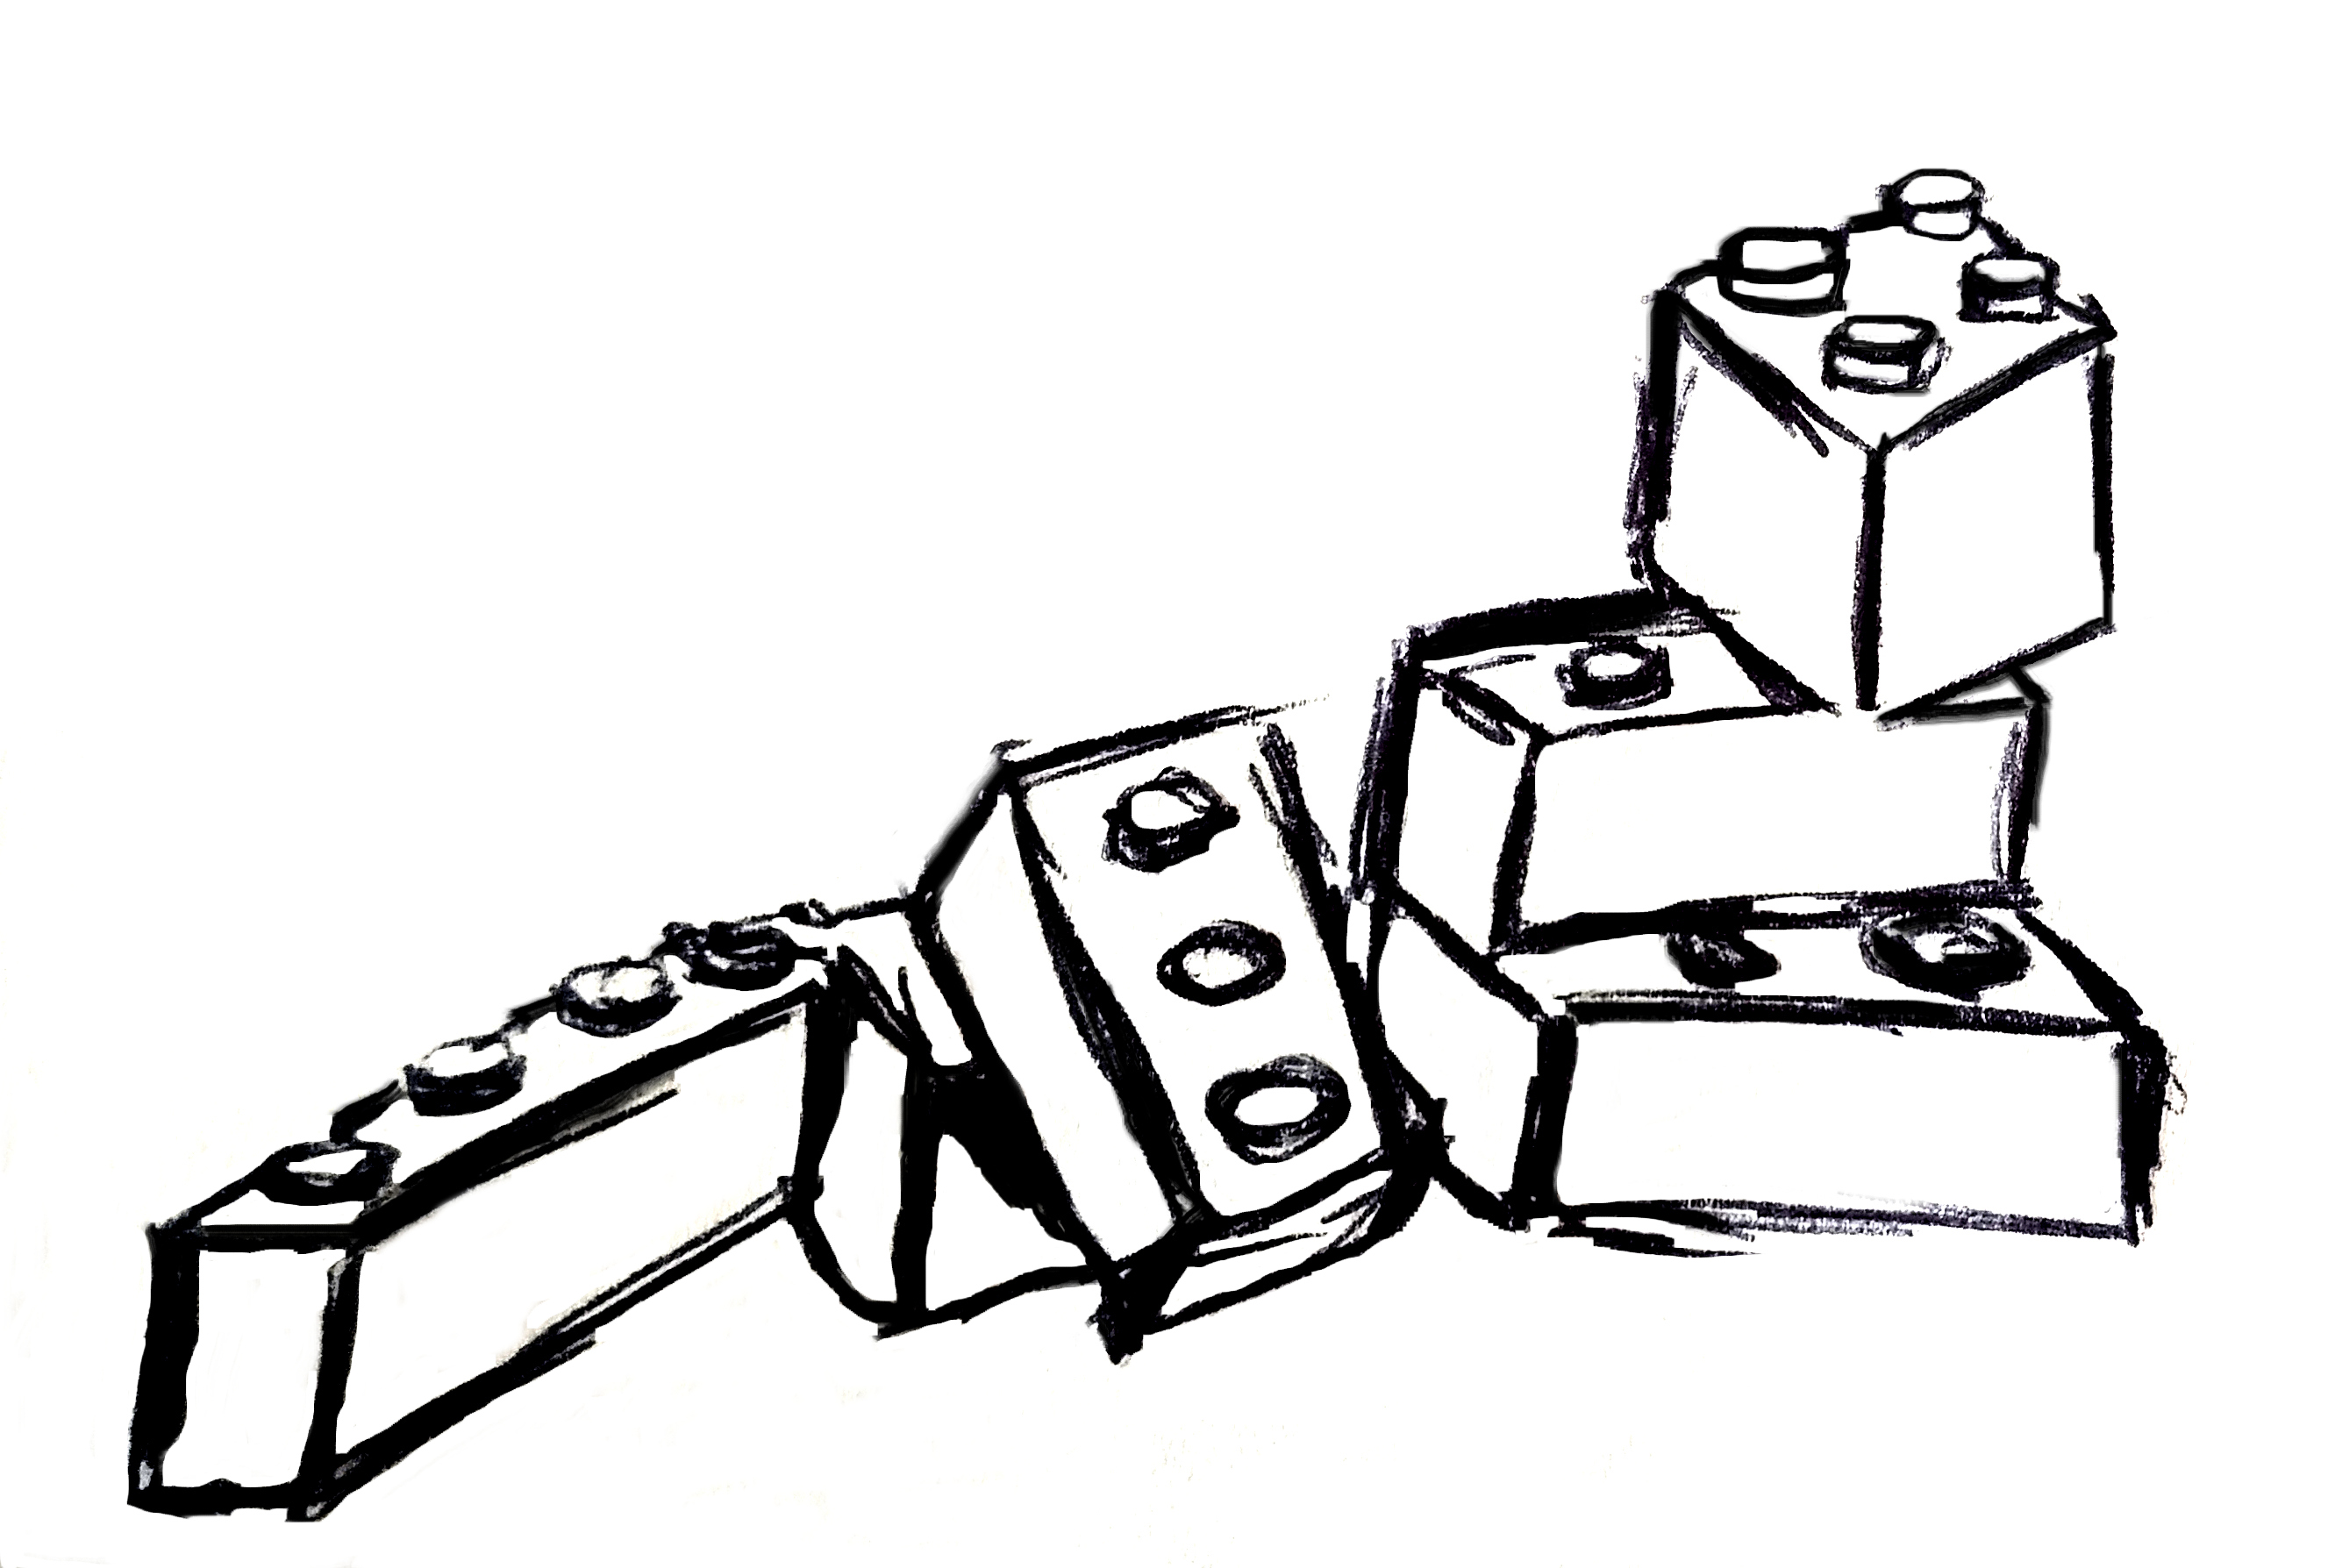
\includegraphics[width=0.4\textwidth]{lego2.jpg}
        \vspace{1cm}
    \end{figure*}

% Idées : plutôt se concentrer sur la SOM en elle-même. Champs d'application, performances, remarquer que les SOM ont des performances pour extraire des représentations, inspi biologique
% Voila ce qui n'a pas été réalisé, et voila ce que je propose : injecter de l'information de position 
% démarche synthétique
% caractériser le comportement émergent des cartes.



% Des systèmes en apparence simples présentent ainsi des capacités d'optimisation de tâches. Le blob est par exemple un être unicellulaire capable de s'étendre sur plusieurs mètres. Uniquement grâce aux communications chimiques opérant au sein de son plasmodium, il est capable de trouver le chemin le plus court dans un labyrinthe entre deux points sur lesquels sont placés de la nourriture \cite{Nakagaki2000IntelligenceMB} ou de retrouver une configuration optimale d'un réseau de transport. Il sont même capables d'apprentissage~: deux entités qui fusionnent se transmettent des connaissances de leur environnement, montrant qu'elles ont chacune emmagasiné, à un point, de l'information sur ce dernier.
% Les colonies de fourmis, quant à elles constituées de milliers, voire de millions d'individus, sont capables de s'auto-organiser pour effectuer des tâches complexes de coopération pour construire leur nid, se défendre face aux prédateurs et trouver leur nourriture via une communication par leurs phéromones, son et toucher.
% Autrement dit, ces systèmes biologiques présentent des capacités de calcul remarquables. 
% Toutes ces stratégies mises en place par des systèmes biologiques ont inspiré de nombreux algorithmes d'optimisation imitant par exemple les colonies de fourmis, les essaims d'abeilles, les groupes de chats, les bancs de poissons ou encore les baleines, tous ces groupes d'animaux présentant des méthodes de communication décentralisées efficaces pour accomplir une tâche donnée~\cite{Darwish2018BioinspiredCA}.




% Les réseaux de neurones impulsionnels (\emph{Spiking Neural Networks}) sont un exemple de modèle d'apprentissage illustrant une complémentarité récente entre l'approche bio-inspirée et l'approche computationnelle.
% Ces réseaux de neurones ont été développés dès les années 1990~\cite{Maass1996NetworksOS} et s'appuient directement sur le modèle biologique du neurone.
% Ils apparaissent dans de nombreux travaux récents comme une méthode montante dans le domaine de l'apprentissage automatique pour la conception de modèles d'apprentissage moins énergivores et distribués, grâce à la conception d'architectures matérielles neuromorphiques telles que LOIHI \footnote{\url{https://www.intel.com/content/www/us/en/research/neuromorphic-computing.html}}. De nombreux travaux cherchent ainsi à adapter des réseaux de neurones classiques de l'état de l'art dans une version impulsionnelle, faisant ainsi passer les SNN de la biologie au calcul~\cite{Schuman2022OpportunitiesFN}.
% De tels modèles apportent de nouveaux paradigmes de calcul pouvant se combiner avec des approches plus appliquées.
% Nous pensons ainsi qu'il est pertinent de continuer à explorer des modèles d'apprentissage automatique inspirés de la biologie.

%Exemples ?
% Le blob est par exemple un être unicellulaire capable de s'étendre sur plusieurs mètres. Uniquement grâce aux communications chimiques opérant au sein de son plasmodium, il est capable de trouver le chemin le plus court dans un labyrinthe entre deux points sur lesquels sont placés de la nourriture \cite{Nakagaki2000IntelligenceMB} ou de retrouver une configuration optimale d'un réseau de transport. Ils sont même capables d'apprentissage~: deux entités qui fusionnent se transmettent des connaissances de leur environnement, montrant qu'elles ont chacune emmagasiné, à un point, de l'information sur ce dernier.
% Les colonies de fourmis, quant à elles constituées de milliers, voire de millions d'individus, sont capables de s'auto-organiser pour effectuer des tâches complexes de coopération pour construire leur nid, se défendre face aux prédateurs et trouver leur nourriture via une communication par leurs phéromones, son et toucher.

%Le perceptron, modèle à l'origine des réseaux de Deep Learning les plus performants à l'heure actuelle, s'inspirait par exemple d'un modèle de neurone biologique très simplifié~\parencite{McCulloch1990ALC}.
% Les réseaux de neurones impulsionnels (\emph{Spiking Neural Networks}) sont un exemple de modèle d'apprentissage illustrant une complémentarité récente entre l'approche bio-inspirée et l'approche computationnelle. Ces réseaux de neurones inspirés du codage temporel des populations de neurones ont été développé dans les années 90~\parencite{Maass1996NetworksOS}. Il apparaissent cependant dans de nombreux travaux récents comme une méthode montante dans le domaine de l'apprentissage automatique pour la conception systèmes d'apprentissage moins énergivores et distribués grâce à la conception de nouvelles architectures matérielles neuromorphiques telles que LOIHI \footnote{\url{https://www.intel.com/content/www/us/en/research/neuromorphic-computing.html}}.
% %\cite{Yamazaki2022SpikingNN}
% L'inspiration biologique apporte ainsi de nouveaux paradigmes de calcul pouvant se combiner avec des approches plus appliquées, et évoluant avec les progrès techniques et matériels de l'informatique.